% proposal skripsi.
\documentclass{jtetiproposalskripsi}

%-----------------------------------------------------------------
%Disini awal masukan untuk data proposal skripsi
%-----------------------------------------------------------------
\titleind{Qos (Quality of service) pada jaringan CCTV berbasis OpenWrt}

\fullname{FUAD HARIS}

\idnum{1210652003}

\approvaldate{06 Januari 2015}



\yearsubmit{2015}

\program{Teknik Informatika}



\dept{Teknologi Informasi}


\begin{document}

\cover

%\approvalpage

%-----------------------------------------------------------------
%Disini akhir masukan untuk muka skripsi
%-----------------------------------------------------------------

%-----------------------------------------------------------------
%Disini awal masukan Intisari
%-----------------------------------------------------------------
\begin{abstractind}
Pada jaman sekarang cctv banyak digunakan untuk berbagai macam keperluan sebuah instansi, biasanya digunakan untuk mengawasi dan merekam suatu aktivitas dalam suatu area/lokasi baik berupa aset perusahaan maupun karyawan. Pengawasan dapat dilakukan dimana saja secara realtime jika terhubung dengan internet, supaya pengawasan berjalan lancar perlu ada network monitoring untuk memonitor lalu lintas dari jaringan, QoS terdiri dari throughput, delay dan packet loss.

\bigskip
\textbf{Kata kunci} : \emph{QOS}, \emph{CCTV}, \emph{OpenWrt}
\end{abstractind}
%-----------------------------------------------------------------
%Disini akhir masukan Intisari
%-----------------------------------------------------------------

\tableofcontents
\addcontentsline{toc}{chapter}{DAFTAR ISI}
\selectlanguage{bahasa}\clearpage\pagenumbering{arabic}\setcounter{page}{1}

%-----------------------------------------------------------------
%Disini awal masukan untuk Bab
%-----------------------------------------------------------------
\chapter{LATAR BELAKANG}

\section{Latar Belakang Masalah}
CCTV  banyak digunakan dalam sebuah instansi untuk memonitoring suatu kegiatan didalam ruangan maupun diluar ruangan,cctv menggunakan teknologi kamera yang terkoneksi dengan digital video recorder (DVR) menggunakan kabel coaxial maupun utp,dari DVR kita koneksikan ke perangkat modem/ bisa lebih dulu ke router yang berbasiskan openwrt,dari openwrt kita atur Qossupaya hasil monitoring lewat internet lebih bagus. Qos terdiri dari throughput, delay dan packet loss. Dibeberapa instansi lebih banyak menggunakan cctv dengan koneksi internet biasa tanpa ada pengontrol bandwith atau Qos, sehingga berpengaruh ketika melakukan monitoring lewat internet,dari masalah tersebut munculah gagasan untuk menggunakan qos pada jaringan cctv supaya lebih tepat dan sesuai dalam pemakaian bandwidth. 

\section{Tujuan Penelitian}
Supaya kualitas jaringan CCTV yang dimonitoring lewat internet lebih bagus dan sesuai kebutuhan menggunakan metode Qos dengan memakai firmware berbasiskan Opensource yaitu OpenWrt.



\section{Manfaat Penelitian}
Kegiatan monitoring menjadi lebih lancar dimanapun berada,pemakaian bandwidth yang tepat sesuai dengan kebutuhan.

%-------------------------------------------------------------------------------
\chapter{TINJAUAN PUSTAKA DAN DASAR TEORI}                

\section{QOS (Quality of Service)}
QoS adalah kemampuan suatu jaringan untuk menyediakan layanan yang baik dengan menyediakan bandwith, mengatasi jitter dan delay. Parameter QoS adalah latency, jitter, packet loss, throughput, MOS, echo cancellation dan PDD. QoS sangat ditentukan oleh kualitas jaringan yang digunakan. Terdapat beberapa faktor yang dapat menurunkan nilai QoS, seperti : redaman, distorsi, dan noise (Fatoni 2011).
Parameter QoS adalah :

Packet loss
	Merupakan suatu parameter yang menggambarkan suatu kondisi yang menunjukkan jumlah total paket yang hilang, dapat terjadi karena collision dan congestion pada jaringan dan hal ini berpengaruh pada semua aplikasi karenaretransmisi akan mengurangi efisiensi jaringan secara keseluruhan meskipun jumlah bandwidth cukup tersedia untuk aplikasi aplikasi tersebut.
	
	Delay
	Adalah waktu yang dibutuhkan data untuk menempuh jarak dari asal ke tujuan. Delay dapat dipengaruhi oleh jarak, media fisik, kongesti atau juga waktu proses yang lama.
	 
Jitter
lazimnya disebut variasi delay ,berhubungan erat dengan latency, yang menunjukkan banyaknya variasi delay pada taransmisi data di jaringan. Delayantrian pada router dan switch dapat menyebabkan jitter

Throughput
Yaitu kecepatan (rate) transfer dataefektif, yang diukur dalam bps.Throughput merupakan jumlah total kedatangan paket yang sukses yang diamati pada tujuan selama interval waktu tertentu dibagi oleh durasi interval waktu tersebut.

Mean Opinion Source (MOS)
Kualitas sinyal yang diterima biasanya diukur secara subjektif dan objektif. Metoda pengukuran subjektif yang umum dipergunakan dalam pengukuran kualitas speech coder adalah ACR (Absolute Category Rating) yang akan menghasilkan nilai MOS. Tes subyektif ACR meminta pengamat untuk menentukan kualitas suatu speech coder tanpa membandingkannya dengansebuah referensi. Skala rating umumnya mempergunakan penilaian yaitu berturut-turut: Exellent, Good, Fair, Poor dan Bad dengan nilai MOS berturut-turut: 5, 4, 3, 2 dan 1. Kualitas suara minimum mempunyai nilai setara MOS 4.0


\section{OpenWrt}
OpenWrt adalah sebuah proyek open source untuk menciptakan sebuah sistem operasi gratis (sebenarnya lebih tepat disebut firmware) yang bisa di install (lebih tepatnya ditanam/ di-embedded) pada perangkat radio wireless. Karena dibuat dengan kernel linux maka Openwrt bisa sebut sebagai salah satu distro linux untuk perangkat embedded (embedd devices).

\section{Kamera CCTV}
Video surveillance System atau disebut Closed Circuit Television System berfungsi mengontrol semua kegiatan secara visual (audio visual) pada area tertentu yang dipasang suatu alat berupa kamera, yang fungsinya secara langsung dapat mengawasi dan mengamati serta merekam kejadian di suatu tempat, ruangan atau area tertentu. Alat ini terdiri dari kamera, digital video recorder dan monitor yang terintegrasi dalam suatu sistem jaringan secara online (CCTV, 2011).Keuntungan Penggunaan CCTV :

Keamanan CCTV merupakan alat pengawas terus menerus dan tidak mengenal lelah. CCTV juga berfungsi preventif karena secara psikologis orang menjadi takut dan enggan untuk berbuat yang jahat karena setiap orang mengetahui benar ada kamera pengawas yang selalu dapat mengawasi gerak-gerik setiap orang yang di rasa mencurigakan. Disisi lain gerak-gerik orang yang mencurigakan dapat diawasi petugas security dari ruang monitor agar bisa secara cepat memutuskan dalam mengambil tindakan, keterbatasan jumlah petugas keamanan yang terbatas pun bisa sangat terbantu dengan adanya CCTV.

Alat bukti yang jujur dan kuat. Jika terjadi tindak kejahatan dan hal tersebut terekam oleh kamera, maka kita dapat dengan mudah mencari rekaman pada jam, tanggal dan hari tertentu untuk digunakan sebagai alat bukti untuk mencari pelaku kejahatan.

Alat peningkatan kinerja karyawan. Dengan adanya penempatan kamera CCTV pada ruang atau gudang tempat kerja maka secara psikologis karyawan akan selalu merasa diawasi oleh atasannya yang tidak selalu berada di tempat. Disamping itu seorang atasan bisa merekam efektivitas kerja karyawan saat karyawan tidak berada di ruangan. Baik saat jam kerja atau pada sore hari sehingga hari berikutnya bisa di playback.

Alat marketing dalam hal keamanan, modern dan profesional. CCTV sudah merupakan salah satu standar keamanan dengan teknologi modern yang harus dimiliki oleh perusahaan-perusahaan publik yang mengutamakan kepuasan pelanggan/ pembeli karena dengan adanya CCTV akan menambah rasa aman dan nyaman yang diberikan oleh pengelola gedung. Adanya CCTV juga bisa menjadi salah satu indikasi bagi calon pelanggan/ pembeli bahwa pengelola gedung juga mengelola keamanan gedungnya dengan cara professional. Contoh nyata jika CCTV system dipasang pada area perparkiran mobil dan hal tersebut diketahui para pengunjung, pembeli atau pelanggan maka para calon pembeli pasti akan lebih merasa aman memarkir kendaraan mereka dan meninggalkan mobilnya di area perpakiran.

CCTV dipasang di kantor cabang maka dengan melalui jaringan yang ada kejadian tersebut bisa juga dilihat di kantor pusat atau pengawasan pada proses transaksi di tempat yang kita inginkan asalkan ada jaringan serta sudah diisntall software sistemnya makan akan dilihat proses transaksi tersebut.

Empat teknik umum yang digunakan untuk meningkatkan kualitas layanan pada jaringan komputer, yaitu:

Penjadwalan (Scheduling)
Paket dari aliran data yang berbeda sampai di router dan switch untuk diproses. Teknik penjadwalan yang baik memperlakukan aliran data yang berbeda secara tepat dan adil. Tiga teknik penjadwalan yang didesain untuk meningkatkan kualitas pelayanan, yaitu :

FIFO Queuing
FIFO (First In First Out) merupakan teknik antrian yang menampung paket ke dalam buffer (ruang memori pada switch dan router) hingga node (router dan switch) siap memprosesnya. Jika kecepatan kedatangan rata-rata lebih tinggi dibandingkan kecepatan pemrosesan rata-rata, antrian akan memenuhi buffer dan paket yang baru dating akan diabaikan.

Priority Queuing
Teknik antrian priority queuing membeda-bedakan paket berdasarkan kelas prioritas. Masing-masing prioritas mempunyai antriannya sendiri. Paket dengan antrian prioritas tertinggi akan diproses terlebih dahulu, sedangkan yang rendah akan diproses terakhir. Sistem tidak akan memproses antrian hingga antriannya habis. Teknik ini lebih baik dibandingkan FIFO karena antrian dengan prioritas traffic yang tinggi seperti multimedia dapat sampai ke tujuan dengan delay yang rendah. Namun memiliki kekurangan jika aliran data secara terus menerus pada antrian prioritas tertinggi, maka paket pada antrian prioritas terendah tidak akan pernah berkesempatan untuk diproses. Kondisi ini disebut starvation atau kelaparan.
 
Weighted Fair Queuing
Teknik antrian weighted fair queuing merupakan metode penjadwalan yang lebih baik. Pada teknik ini paket masih dibedakan di kelas dan antrian yang berbeda. Masing-masing prioritas antrian diberi pemberat yang berbeda, dimana prioritas yang lebih tinggi diberi pemberat yang lebih tinggi juga. Sistem akan memproses paket di tiap antrian secara bergantian dengan pemilihan paket di tiap antrian
berdasarkan beratnya. Jika sistem tidak menerapkan prioritas pada kelas-kelasnya maka beratnya dianggap sama (jumlah paket yang diproses sama), dalam hal ini antrian memiliki prioritas yang adil.

Traffic Shaping
Traffic shaping adalah mekanisme untuk mengontrol jumlah dan kecepatan data dari traffic yang dikirimkan ke jaringan. Dua teknik yang digunakan mengontrol traffic :
 
Leaky Bucket
Teknik ini digunakan untuk meratakan input data yang jumlahnya naik turun dalam traffic jaringan (bursty traffic) dengan merata-rata kecepatan data. Bursty yang masuk disimpan ke dalam penampungan (bucket) dan dikelurakan ke jaringan dengan rata-rata kecepatan yang konstan. Teknik ini mencegah kemacetan pada jaringan (congestion network) karena semua paket memiliki kesempatan untuk diproses yang dibedakan berdasarkan jumlah paket yang diproses. Setiap satuan waktu ada paket yang diproses yang kemudian dilepaskan ke dalam jaringan. Jika traffic terdiri dari variable panjang paket yang bervariasi, kecepatan yang dikeluarkan harus sesuai pada jumlah byte atau bit paket tersebut. Algoritma untuk paket dengan panjang paket yang bervariasi :
1. Inisialisasi counter menjadi n pada tiap detik
2. Jika n lebih besar dari ukuran paket, kirim paket dan tambahkan nilai counter dengan ukuran paket. Ulangi langkah 2 hingga n lebih kecil dari ukuran paket
3. Reset counter dan ulangi langkah 1.

Token Bucket
Algoritma teknik token bucket mengijinkan pada host yang tidak memakai jaringan untuk mengumpulkan credit untuk pengiriman selanjutnya dalam bentuk token-token.Untuk tiap detik system mengirimkan sejumlah n token ke bucket (penampungan). Sistem menghilangkan satu token tiap cell (tiap byte) data dikirimkan. Teknik token bucket dengan mudah diimplementasikan dengan counter. Token diinisialisasi menjadi 0. Tiap waktu token ditambahkan, counter ditambahkan 1. Tiap waktu satu unit data dikirimkan counter dikurangi dengan 1. Ketika counter bernilai 0, host tidak bisa mengirimkan data. Teknik token bucket mengijinkan bursty traffic pada kecepatan maksimum yang diijinkan.

Mengkombinasikan Token Bucket dan Leaky Bucket
Dua teknik bisa dikombinasikan memanfaatkan host yang tidak memakai jaringan dan pada saat yang sama mengatur traffic. Leaky Bucket dijalankan setelah Token Bucket, kebutuhan kecepatan leaky bucket (keluarnya token) harus lebih tinggi dari pada kecepatan masuknya token pada bucket. 

Resource Reservation
Resource reservation merupakan penyediaan sumber daya dalam aliran data yang dibutuhkan saat mengirim atau menerima data. Aliran data membutuhkan sumber daya seperti buffer, bandwith, waktu CPU (central processing unit), dsb. Kualitas pelayanan menyediakan sumber daya ini sebelum data ada pada aliran.

Admission Control
Admission control merupakan mekanisme yang digunakan router atau switch untuk menerima atau menolak aliran data yang parameternya ditentukan terlebih dahulu, parameter ini disebut spesifikasi aliran. Sebelum router menerima aliran data untuk diproses, router akan memeriksa spesifikasi aliran untuk melihat kapasitas router (dalam hal ini badwidth, ukuran buffer, kecepatan CPU, dsb) dan ketentuan dengan aliran data yang sebelumnya untuk bisa menangani aliran data yang baru. 

\begin{figure}[ht!]
  \centering
 %   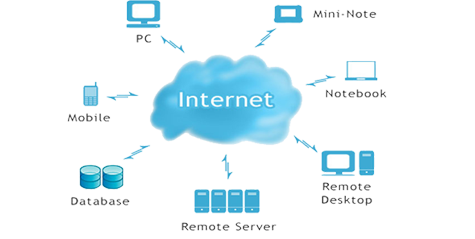
\includegraphics{gambar/star}
    %\caption{Prinsip kerja cloud storage}
    %\label{star}
\end{figure}

%-------------------------------------------------------------------------------
\chapter{METODOLOGI}

\section{Waktu dan tempat}
waktu penelitian dilaksanakan mulai tanggal 6-10 januari 2015 bertempat dikantor kopegtel.


\section{Alat dan Bahan}
\textbf{Perangkat Keras}
\vspace{-0.5cm}
\begin{enumerate}[a.]
\begin{singlespace}
\itemsep0em
\item Acer Aspire 4738 z (1 unit),
\item Tp-link mr3020 (1 unit),
\item Kamera CCTV 
\end{singlespace}
\end{enumerate}

\textbf{Perangkat Lunak}
\vspace{-0.5cm}
\begin{enumerate}[a.]
\begin{singlespace}
\itemsep0em
\item Os Windows 7
\item OpenWrt
\item CCTV avtech
\end{singlespace}
\end{enumerate}


\section{Metodologi Penelitian}
Metode penelitian disini menggunakan metode eksperimen. Metode eksperimen ini bertujuan melakukan penyelidikan yang kemungkinan saling berhubungan antara sebab akibat dengan cara mengenakan kepada satu atau lebih kelompok ekspiremental satu atau lebih kondisi perlakuan dan membandingkan hasilnya dengan satu atau lebih kelompok kontrol yang tidak dikenali kondisi perlakuannya. Suryabrata (2004:88). Dengan mengacu pada model penelitian ini penulis melakukan pendekatan dalam kegiatan penelitian yaitu :

1.Melakukan survey kepustakaan.

2.Mengidentifikasi dan mendefinisikan masalah.

3.Merumuskan hipotesis, berdasarkan atas penelaahan kepustakaan.

4.Mendefinisikan pengertian-pengertian dasar dan variable-variabel utama.

5.Menyusun rencana eksperimen

%-----------------------------------------------------------------
%Disini akhir masukan Bab
%-----------------------------------------------------------------

%-----------------------------------------------------------------
%Disini awal masukan untuk Daftar Pustaka
%-----------------------------------------------------------------
%%\nocite{Abel2010,Guerbas201350}
%%\bibliography{research-plan}
%%\bibliographystyle{plainnat}
\begin{thebibliography}{9}

\bibitem[satu(2013)]{satu01}
Rahayu, 2013. "monitoring dan analisis kualitas layanan trafik kamera cctv pada jaringan wireless".


\end{thebibliography}
\addcontentsline{toc}{chapter}{DAFTAR PUSTAKA}
%-----------------------------------------------------------------
%Disini akhir masukan Daftar Pustaka
%-----------------------------------------------------------------

\end{document}